%%%
%%%%%%%%%%%%%%%%%%%%%%%%%%%%%%%%%%%%%%%%%%%%%%%%%%%%%
%%% Draft paper for Diversity, Equity, and Inclusion in HRI
%%% https://sites.google.com/view/dei-hri/call-for-papers
%%% Important dates 
%%% Deadline January 30th, 2023 (final extension)
%%% Paper Acceptance Notification: February 13th, 2023 (final extension)
%%% Camera-Ready Paper: March 1st, 2023
%%%
%%%
%%%%%%%%%%%%%%%%%%%%%%%%%%%%%%%%%%%%%%%%%%%%%%%%%%%%%
%%% Roadmap for dei-hri2023:
%%% 1. Setting template and draft sections: 14-to-15-Jan-2023
%%% 2. Distillation: 15-to-20-Jan
%%% 3. 25min-ish google-meeeting: 19-Jan 15:00/Mex; 21:00/UK; 13:00/Vancouver; 22:00/Spain; 13:00/PST 
%%% 4. Send second draft Friday 20th Jan
%%% 5. Submission: 23th Jan 2023: 
%%%
%%%
%%%
%%%%%%%%%%%%%%%%%%%%%%%%%%%%%%%%%%%%%%%%%%%%%%%%%%%%%
%%% Overleaf project
%%% Anyone with this link can edit this project
%%% https://www.overleaf.com/3395627816xdvrymdbqqft
%%%
%%%%%%%%%%%%%%%%%%%%%%%%%%%%%%%%%%%%%%%%%%%%%%%%%%%%%
%%% Instrucitons for overleaf project
%%% Overleaf might be new to you, but it is quite easy to use. 
%%% 1. Go to the section where you want to write up in the PDF paper and double click that will point you to the text editor. 
%%% 2. Make edition as in word, and
%%% 3. Prese Ctrl+s to save and compile your changes in the PDF document.
%%% 4. After Ctrl+s, all should be saved and ready for others to see, to review, etc.
%%% Ps. Using percentage symbol is consdiered as comment and it is not apearing in the PDF version of the paper.
%% Don't worry about adding new references `\cite{}`, we can add them later.
%%% Thanks, Miguel
%%%
%%%
%%%%%%%%%%%%%%%%%%%%%%%%%%%%%%%%%%%%%%%%%%%%%%%%%%%%%
%%% Github project:
%%% https://github.com/air4children/dei-hri2023/  
%%%
%%%
%%%
%%%
%%%

%%%%%%%%%%%%%%%%%%%%%%%%%%%%%%%%%%%%%%%%%%%%%%%%%%%%%
%% This is file `main.tex',
%% generated with the docstrip utility.
%%
%% The original source files were:
%%
%% samples.dtx  (with options: `manuscript')
%% 
%% IMPORTANT NOTICE:
%% 
%% For the copyright see the source file.
%% 
%% Any modified versions of this file must be renamed
%% with new filenames distinct from sample-manuscript.tex.
%% 
%% For distribution of the original source see the terms
%% for copying and modification in the file samples.dtx.
%% 
%% This generated file may be distributed as long as the
%% original source files, as listed above, are part of the
%% same distribution. (The sources need not necessarily be
%% in the same archive or directory.)
%%
%% Commands for TeXCount
%TC:macro \cite [option:text,text]
%TC:macro \citep [option:text,text]
%TC:macro \citet [option:text,text]
%TC:envir table 0 1
%TC:envir table* 0 1
%TC:envir tabular [ignore] word
%TC:envir displaymath 0 word
%TC:envir math 0 word
%TC:envir comment 0 0
%%
%%
%% The first command in your LaTeX source must be the \documentclass command.
%%%% Small single column format, used for CIE, CSUR, DTRAP, JACM, JDIQ, JEA, JERIC, JETC, PACMCGIT, TAAS, TACCESS, TACO, TALG, TALLIP (formerly TALIP), TCPS, TDSCI, TEAC, TECS, TELO, THRI, TIIS, TIOT, TISSEC, TIST, TKDD, TMIS, TOCE, TOCHI, TOCL, TOCS, TOCT, TODAES, TODS, TOIS, TOIT, TOMACS, TOMM (formerly TOMCCAP), TOMPECS, TOMS, TOPC, TOPLAS, TOPS, TOS, TOSEM, TOSN, TQC, TRETS, TSAS, TSC, TSLP, TWEB.
% \documentclass[acmsmall]{acmart}

%%%% Large single column format, used for IMWUT, JOCCH, PACMPL, POMACS, TAP, PACMHCI
% \documentclass[acmlarge,screen]{acmart}

%%%% Large double column format, used for TOG
% \documentclass[acmtog, authorversion]{acmart}

%%%% Generic manuscript mode, required for submission
%%%% and peer review

%\documentclass[manuscript,screen,review]{acmart}
%\documentclass[sigconf,authordraft]{acmart}
%\documentclass[sigconf,review]{acmart}
\documentclass[sigconf,anonymous,review]{acmart}
%\documentclass[sigconf,review]{acmart}
%\documentclass[sigchi-a,anonymous,review]{acmart}
%\documentclass[acmconf,anonymous,review]{acmart}

%sigchi: Used for SIGCHI conference articles.
%sigchi-a: Used for SIGCHI “Extended Abstract” articles.
%sigplan: Used for SIGPLAN conference articles.


\graphicspath{{../figures}} %goes to path: figures/

%% Fonts used in the template cannot be substituted; margin 
%% adjustments are not allowed.
%%
%% \BibTeX command to typeset BibTeX logo in the docs
\AtBeginDocument{%
  \providecommand\BibTeX{{%
    \normalfont B\kern-0.5em{\scshape i\kern-0.25em b}\kern-0.8em\TeX}}}

%% Rights management information.  This information is sent to you
%% when you complete the rights form.  These commands have SAMPLE
%% values in them; it is your responsibility as an author to replace
%% the commands and values with those provided to you when you
%% complete the rights form.
\setcopyright{acmcopyright}
\copyrightyear{2023}
\acmYear{2023}
\acmDOI{XXXXXXX.XXXXXXX}

%% These commands are for a PROCEEDINGS abstract or paper.
\acmConference[HRI '23]{Make sure to enter the correct
  conference title from your rights confirmation emai}{March 13--16,
  2023}{Stockholm, SE}
%
%  Uncomment \acmBooktitle if th title of the proceedings is different
%  from ``Proceedings of ...''!
%
\acmBooktitle{HRI '23: ACM/IEEE International Conference on Human-Robot Interaction, 
March 13-16, 2023 Stockholm, SE} 
\acmPrice{15.00}
\acmISBN{978-1-4503-XXXX-X/18/06}


%%
%% Submission ID.
%% Use this when submitting an article to a sponsored event. You'll
%% receive a unique submission ID from the organizers
%% of the event, and this ID should be used as the parameter to this command.
%%\acmSubmissionID{123-A56-BU3}

%%
%% For managing citations, it is recommended to use bibliography
%% files in BibTeX format.
%%
%% You can then either use BibTeX with the ACM-Reference-Format style,
%% or BibLaTeX with the acmnumeric or acmauthoryear sytles, that include
%% support for advanced citation of software artefact from the
%% biblatex-software package, also separately available on CTAN.
%%
%% Look at the sample-*-biblatex.tex files for templates showcasing
%% the biblatex styles.
%%

%%
%% The majority of ACM publications use numbered citations and
%% references.  The command \citestyle{authoryear} switches to the
%% "author year" style.
%%
%% If you are preparing content for an event
%% sponsored by ACM SIGGRAPH, you must use the "author year" style of
%% citations and references.
%% Uncommenting
%% the next command will enable that style.
%%\citestyle{acmauthoryear}

%%
%% end of the preamble, start of the body of the document source.
\begin{document}

%%
%% The "title" command has an optional parameter,
%% allowing the author to define a "short title" to be used in page headers.
\title{
%How to teach bias in AI and Robotics to Mexican Children?%Sun 15 Jan 07:22:56 GMT 2023
% Teaching bias in AI and Robotics to Mexican Children%Sun 15 Jan 08:25:41 GMT 2023
%Teaching bias in AI and Robotics to Children in a small community in Mexico
%Fri 20 Jan 06:15:26 GMT 2023
Teaching AI and Robotics to Children in a Mexican town
%Mon 23 Jan 23:57:27 GMT 2023
}

%%
%% The "author" command and its associated commands are used to define
%% the authors and their affiliations.
%% Of note is the shared affiliation of the first two authors, and the
%% "authornote" and "authornotemark" commands
%% used to denote shared contribution to the research.
\author{Ben Trovato}
\authornote{Both authors contributed equally to this research.}
\email{trovato@corporation.com}
\orcid{1234-5678-9012}
\author{G.K.M. Tobin}
\authornotemark[1]
\email{webmaster@marysville-ohio.com}
\affiliation{%
  \institution{Institute for Clarity in Documentation}
  \streetaddress{P.O. Box 1212}
  \city{Dublin}
  \state{Ohio}
  \country{USA}
  \postcode{43017-6221}
}

\author{Lars Th{\o}rv{\"a}ld}
\affiliation{%
  \institution{The Th{\o}rv{\"a}ld Group}
  \streetaddress{1 Th{\o}rv{\"a}ld Circle}
  \city{Hekla}
  \country{Iceland}}
\email{larst@affiliation.org}

\author{Valerie B\'eranger}
\affiliation{%
  \institution{Inria Paris-Rocquencourt}
  \city{Rocquencourt}
  \country{France}
}

\author{Aparna Patel}
\affiliation{%
 \institution{Rajiv Gandhi University}
 \streetaddress{Rono-Hills}
 \city{Doimukh}
 \state{Arunachal Pradesh}
 \country{India}}

\author{Huifen Chan}
\affiliation{%
  \institution{Tsinghua University}
  \streetaddress{30 Shuangqing Rd}
  \city{Haidian Qu}
  \state{Beijing Shi}
  \country{China}}

\author{Charles Palmer}
\affiliation{%
  \institution{Palmer Research Laboratories}
  \streetaddress{8600 Datapoint Drive}
  \city{San Antonio}
  \state{Texas}
  \country{USA}
  \postcode{78229}}
\email{cpalmer@prl.com}

\author{John Smith}
\affiliation{%
  \institution{The Th{\o}rv{\"a}ld Group}
  \streetaddress{1 Th{\o}rv{\"a}ld Circle}
  \city{Hekla}
  \country{Iceland}}
\email{jsmith@affiliation.org}

\author{Julius P. Kumquat}
\affiliation{%
  \institution{The Kumquat Consortium}
  \city{New York}
  \country{USA}}
\email{jpkumquat@consortium.net}

%%
%% By default, the full list of authors will be used in the page
%% headers. Often, this list is too long, and will overlap
%% other information printed in the page headers. This command allows
%% the author to define a more concise list
%% of authors' names for this purpose.
\renewcommand{\shortauthors}{Trovato and Tobin, et al.}

%%
%% The abstract is a short summary of the work to be presented in the
%% article.
\begin{abstract}
In this paper, we present a pilot study aiming to investigate the challenges of teaching AI and Robotics to children in a Mexican town.
Challenges such as teaching bias in AI and inclusive learning with Montessori method were introduced, emphasising the contextual background in Mexico.
For the pilot study, we invited 14 participants of which 10 were able to attend, 6 male and 4 female of (age in years: mean=8 and std=$\pm$1.61) and four instructors of different teaching experiences and skills to young audiences.
We reported results of four-lesson curriculum of teaching AI and Robotics in a community where little to none experts were able to taught such subjects, and the challenges of creating a curriculum that is both inclusive and engaging with Montessori method and low-cost open source robots. 
We concluded that this pilot study helped participants to understand fundamental concepts of AI and Robotics and provided better understanding on financial and logistical challenges to organise a workshop with a major number of participants as potential future work.
\end{abstract}

%%
%% The code below is generated by the tool at http://dl.acm.org/ccs.cfm.
%% Please copy and paste the code instead of the example below.
%%
\begin{CCSXML}
<ccs2012>
     <concept>
         <concept_id>10003120.10003121.10011748</concept_id>
         <concept_desc>Human-centered computing~Empirical studies in HCI</concept_desc>
         <concept_significance>500</concept_significance>
         </concept>
     <concept>
         <concept_id>10003120.10011738.10011776</concept_id>
         <concept_desc>Human-centered computing~Accessibility systems and tools</concept_desc>
         <concept_significance>500</concept_significance>
         </concept>
     <concept>
         <concept_id>10010405.10010489.10010491</concept_id>
         <concept_desc>Applied computing~Interactive learning environments</concept_desc>
         <concept_significance>300</concept_significance>
         </concept>
     <concept>
         <concept_id>10003456.10010927.10010930.10010931</concept_id>
         <concept_desc>Social and professional topics~Children</concept_desc>
         <concept_significance>500</concept_significance>
         </concept>
     <concept>
         <concept_id>10010147.10010178.10010187.10010194</concept_id>
         <concept_desc>Computing methodologies~Cognitive robotics</concept_desc>
         <concept_significance>300</concept_significance>
         </concept>
</ccs2012>
\end{CCSXML}

\ccsdesc[500]{Human-centered computing~Empirical studies in HCI}
\ccsdesc[500]{Human-centered computing~Accessibility systems and tools}
\ccsdesc[300]{Applied computing~Interactive learning environments}
\ccsdesc[500]{Social and professional topics~Children}
\ccsdesc[300]{Computing methodologies~Cognitive robotics}

%%
%% Keywords. The author(s) should pick words that accurately describe
%% the work being presented. Separate the keywords with commas.
\keywords{Child-centred AI, Educational Robotics, Child-robot interaction}

%% A "teaser" image appears between the author and affiliation
%% information and the body of the document, and typically spans the
%% page.
\begin{teaserfigure}
    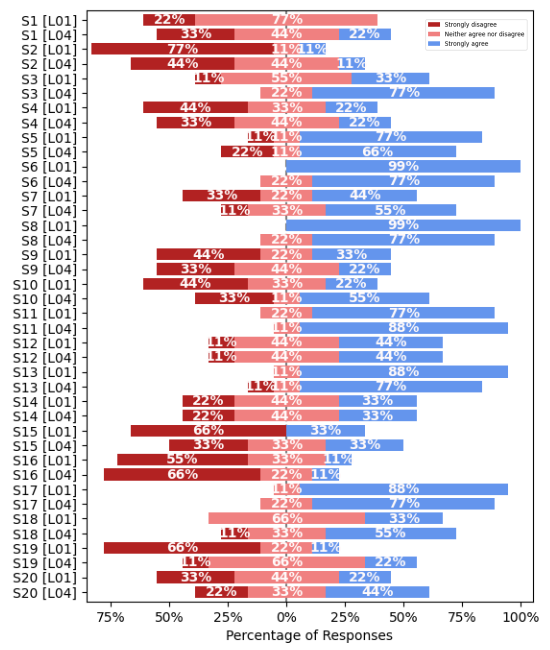
\includegraphics[width=\textwidth]{../figures/main/outputs/drawing-v03.png} %%GITHUB
    % \includegraphics[width=\textwidth]{fig-main.png} %%OVERLEAF
    \caption{
    (a) Instructor demonstrating coding activities with open-source educational robot,
    (b) instructor showing AI and Robotic-based cards for the bingo game,
    (c) instructors presenting difference concepts of AI and Robotics to children,
    (d) children interacting in group activities, and 
    (e) showcase activity where instructor helped the group of four children to present projects. 
    % (c) Bingo game with key terms like neuron, robot, eye, etc., and 
    % (d) piloting teaching materials with children.
    }
    %\Description{}
    \label{fig:main}
\end{teaserfigure}

%%%%%%%%%%%%%%%%%%%%%%%%%%%%%%%
%% History of the paper
%\received{23rd January 2023}
%\received[revised]{6th Feb 2023}
%\received[accepted]{1st March 2023}

%%
%% This command processes the author and affiliation and title
%% information and builds the first part of the formatted document.
\maketitle

\section{Introduction}
Teaching Artificial Intelligence (AI) and Robotics to young learners has been made good progress in the last decade \cite{bers2019, druga2019}.
Educational progress has been possible due to the great investment in AI and Robotics in countries such as U.S.A, Germany, Denmark, and Sweden, making those countries and their communities to define core values in AI and Robotics \cite{druga2019}. These raise the question on 
how to adapt such core values from the most to the least privileged environments~\cite{pratyusha2020}. 
For instance, it has been little progress on using open-source  educational robots and the creation of child-centred programs to teach AI and Robotics in low-income countries ~\cite{abadilloperez2022_DEI_HRI2022, montenegro2021air4children}.
However, there are various challenges on teaching AI and Robotics to young learners such as the barrier of teaching programming skills to those who are still learning writing and reading skills to which visual and auditory programs using sensor, action and logic blocks helped to address such challenges \cite{long2020, wyeth2008}.
Other challenge is the little to none experts to teach AI and Robotics and its limited educational material in low-income countries~\cite{yang2022, abadilloperez2022_DEI_HRI2022}.
% Even though open-source educational robots seems to be affordable, there seems to be
% Current research lines in AI and Robotics claims to be neutral where data pipelines align with principles of findability, accessibility, interoperability, and reusability (FAIR). %TOADD_REF
There is also emerging values in the field of ML/AI on societal forces questioning what research is done and who benefits~\cite{birhane2022}. 
Hence, the aim of this work is to
investigate further challenges of teaching AI and Robotics to young audiences in a Mexican town where little no experts can teach such subjects with limited resources.

%% Here to add a brieft description of the sections of the paper 
In this paper, we present challenges of teaching AI and Robotics to Children in a Mexican town, including study design and curriculum design and results and surveys from a pilot experiment of four lessons and conclusions and future work.

%%%%%%%%%%%%%%%%%%%%%%%%%%%%%%%%%%%%%%%%%%%%%%%%%%%%%%%%%%%%%%%%%%%%%
%% VICTOR to review papers and add summary on the challenges on AI literacy
%Touretzky, D., Gardner-McCune, C., Martin, F. and Seehorn, D. (2019) %Envisioning AI for K12: What should every child know about AI? The Thirty-%Third AAAI Conference on Artificial Intelligence (AAAI-19).
%Introducing the Fundamentals of Artificial Intelligence to K-12 Classrooms %According to Educational Neuroscience Principles
% Perhaps cite papers in the 
%https://www.bcu.ac.uk/education-and-social-work/research/news-and-events/cspace-conference-2021/blog/ai-literacy-the-role-primary-education
%
%See https://stefania11.github.io/assets/pdf/FABLEARN_Inclusive_AI_2019.pdf
%\cite{druga2019} 
%
%%%%%%%%%%%%%%%%%%%%%%%%%%%%%%%%%%%%%%%%%%%%%%%%%%%%%%%%%%%%%%%%%%%%%

\section{Challenges of teaching AI and Robotics to Children}
\subsection{Teaching bias in AI}
Smith et al. pointed out the current challenges of when and how to teach computing ethics to students~\cite{smith2022incorporating}.
Learning ethics in introductory courses help students to think ethically about their computation topics~\cite{fiesler2021}.
% TOREVIEW \cite{weerts2022}
Payne et al. have shown great progress on making pilots and beta test teaching ethical AI to young audiences~\cite{payne2020}.
For instance, on summer 2021 a pilot to teach ethical AI to young audiences were organised with 28 kids at the Media Lab with a cost of \$150 for the week, leading to a beta test with 250 students in autumn 2021. Such pilots considered question related to the everyday life of children, such as 
"What's is the best algorithm to make a peanut-butter sandwich?: is it the algorithm that makes the tastiest sandwich? , is it the prettiest sandwich?, is it the quickest and easiest to make? or the easiest to clean up?". Hence the challenge is how to contextualise such questions in Mexican town where children may know little to know about AI and Robotics or terminology in ethics (bias).
% https://www.wgbh.org/news/science-and-technology/2019/07/31/teaching-kids-the-ethics-of-artificial-intelligence
% https://qz.com/1700325/mit-developed-a-course-to-teach-tweens-about-the-ethics-of-ai

% Immediately following this sentence is the point at which
% Table~\ref{tab:freq} is included in the input file; compare the
% placement of the table here with the table in the printed output of
% this document.
% \begin{table}
%   \caption{Frequency of Special Characters}
%   \label{tab:freq}
%   \begin{tabular}{ccl}
%     \toprule
%     Non-English or Math&Frequency&Comments\\
%     \midrule
%     \O & 1 in 1,000& For Swedish names\\
%     $\pi$ & 1 in 5& Common in math\\
%     \$ & 4 in 5 & Used in business\\
%     $\Psi^2_1$ & 1 in 40,000& Unexplained usage\\
%   \bottomrule
% \end{tabular}
% \end{table}

% Immediately following this sentence is the point at which
% Table~\ref{tab:commands} is included in the input file; again, it is
% instructive to compare the placement of the table here with the table
% in the printed output of this document.

% \begin{table*}
%   \caption{Some Typical Commands}
%   \label{tab:commands}
%   \begin{tabular}{ccl}
%     \toprule
%     Command &A Number & Comments\\
%     \midrule
%     \texttt{{\char'134}author} & 100& Author \\
%     \texttt{{\char'134}table}& 300 & For tables\\
%     \texttt{{\char'134}table*}& 400& For wider tables\\
%     \bottomrule
%   \end{tabular}
% \end{table*}



%%%%%%%%%%%%%%%%%%%%%%%%%%%%%%%%%%%%%%%%%%%%%%%%%%%%%%%%%%%%%%%%%%%
%%CHIO please help to review, to change or to add to the following section
\subsection{Inclusive learning of AI and Robotics with Montessori method}
Montessori method is focused in child-centred development where the role of Montessori teachers is to help children individually or in small groups engaging in self-directed activities \cite{Aljabreen2020}.
The adoption of technological topics (AI and Robotics) into Montessori methods has been experimented and studied in the last 10 years \cite{elkin2014}. 
However, there are other skills that are also required to create inclusive learning of new technologies. For example, "collaborative skills" and "understating concepts" are two main factors to design inclusive AI literary for children in low, medium and high socioeconomic backgrounds \cite{druga2019}. 
Also, there is evidence on the impact of collaboration and engagement activities on how coding games and robots to enhance computational thinking \cite{sharma2019}.
Hence, the challenge is how to adapt Montessori method to not only create conditions to develop physical and social requirements but collaborative and literacy skills through hands-on activities. 

\section{Pilot study: study design and curriculum design}
%%%%%%%%%%%%%%%%%%%%%%%%%%%%%%%%%%%%%%%%%%%%%
% Brieft introduction to this section [MX/TB]
\subsection{Participants}
In this pilot study, we invited 14 participants between the age of 6 to 9 years old. During the pilot workshop, only 10 participants 6 male and 4 female of (age in years: mean=8 and std=$\pm$1.61) were able to join the workshops as remained ones 
  were unable to attend due to personal circumstances. We also invited four instructors with different years of experience in teaching subjects to young audiences and one person to lead the logistics of the event. 

\subsection{Lessons}
Aiming to create inclusive teaching practices for students, we considered a study design based on procedures, instruments,  data collection and analysis~\cite{du2022}.
%%%%%%%%%%%%%%%%%%%%%%%%%%%%%%%%%%%%%%%%%%%%%
%% TON~O and DONATO will draft details of the lessons in four paragraphs (or one large paragraph) 
For instance, Figure~\ref{fig:curriculum} illustrates the curriculum design for the pilot experiment. 
In lesson 01, we introduced basics concept of human senses and how artificial intelligence relates to identifying cats and dogs. We were able to use more dynamic activities with protoboards and simple electric circuits so that children can easily learn fundamentals on how a robot works (Figure~\ref{fig:main}d). 
In lesson 02, we presented examples on how artificial intelligence learn to recognize animals or humans with a tangram activity and gave them a mini introduction to the code that they will use for the robot.
In lesson 03, we adopted a bingo game with key terms from the previous lessons (Figure~\ref{fig:main}b). We 
introduced what is algorithm with an activity of cooking quesadillas where students learnt that everyone can have a different answer given the same instruction.
We also organised activities on action/reaction with different sensors, how sensors work, how to program sensors and examples with the protoboards and circuits.
In lesson 04, we closed the course, starting with an activity in the garden where students program their teammates and practice to give instructions to a robot in order to get the wanted result. Then we show them some real life applications of AI and robotics and we grouped participants in three teams so they could program their robots and design their logo (Figure~\ref{fig:main}e). 
\begin{figure}[h]
  \centering
    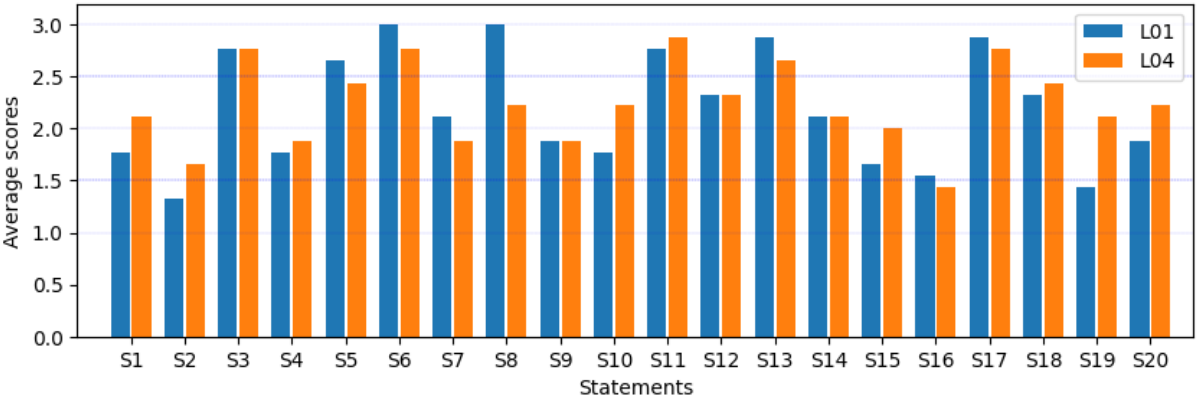
\includegraphics[width=\linewidth]{../figures/curriculum/outputs/drawing-v01.png}  %%GITHUB
    % \includegraphics[width=\linewidth]{fig-curriculum.png}  %%OVERLEAF
    \caption{
    Curriculum design with four lessons of 1 hour and a half 
 (L01, L02, L03 and L04).
    The arrows illustrate the connection between the first and the last part of each lessons as way to summarise the progress of each lesson and the full curriculum.
    }
    \label{fig:curriculum}
\end{figure}

\section{Results}
% \subsection{Pilot study}
Four lessons of the curriculum were organised on Mondays and Wednesdays in two weeks of November 2022. 
Instructors helped children in the pilot workshop by creating groups of three to four children.
In the final lesson groups presented their project with their own robot and children with the help of the instructor explained the application of the robot.


\begin{figure}[h]
  \centering
    \includegraphics[width=\linewidth]{../figures/results/outputs/drawing-v00.png}  %%GITHUB
    % \includegraphics[width=\linewidth]{fig-results.png}  %%OVERLEAF
    \caption{
    Results of the survey with 20 statements (s1, to s20) of 10 participants of the workshop. Please see appendix A for further references on the statements of the survey.
    NOTE. RESULTS FOR 23-NOV NEEDS TO BE ADDED!
    }
    \label{fig:results}
\end{figure}
% \subsection{Surveys}
% TODO

\section{Conclusions and future work}
%%%%%%%%%%%%%%%%%%%%%%%%
%%% CONCLUSIONS
%%% Please add any conclusions that you saw during the pilot
In this paper, we investigated the challenges of teaching AI and Robotics to young audiences with a pilot study in a Mexican town. We concluded that Parents and children have the willingness to join this pilot study by participating and learning new experiences on collaborative and fun activities with low-cost educational robots. However, limited self-funded budget restricted us to prepare and  organised a major number of lessons and reach more participants which hopefully will be addressed in future work.
%%%%%%%%%%%%%%%%%%%%%%%%
%%%FUTURE WORK
%%% please add your initials and paragraphs on what you might consider be a good line of research for future work.
%% MX: How to incorporate other examples of bias in AI/Robotics in the context of the Mexican society?
%%




%% The acknowledgments section is defined using the "acks" environment
%% (and NOT an unnumbered section). This ensures the proper
%% identification of the section in the article metadata, and the
%% consistent spelling of the heading.
\begin{acks}
To everyone involved in this collaborative work.
\end{acks}

%%
%% The next two lines define the bibliography style to be used, and
%% the bibliography file.
\bibliographystyle{ACM-Reference-Format}
\bibliography{../references/references} %%GITHUB
% \bibliography{references} %%OVERLEAF

%%%
%%% If your work has an appendix, this is the place to put it.
\appendix

\section{Surveys}
Figure~\ref{fig:survey} shows survey layout document and 
table \ref{tab:questions} presents 20 statements of the survey.

\begin{table*}
  \caption{Statements in the survey}
  \label{tab:questions}
  \begin{tabular}{ll}
    \toprule
    Number & Statements \\
    \midrule
    S1 & I would enjoy being a scientist when I grow up \\
    S2 & I would enjoy being an engineer when I grow up.  \\
    S3 & I would like a job where I could invent things. \\
    S4 & I would like to help to plan bridges, skyscrapers, and tunnels. \\
    S5 & I would like a job that lets me design a cars. \\   
    S6 & I would like to build and test machines that could help people to walk. \\
    S7 & I would enjoy a job helping to make new medicines. \\
    S8 & I would enjoy a job helping to protect the environment. \\
    S9 & Science has nothing to do with real life. \\
    S10 & Math has nothing to do with real life. \\
    S11 & I would like a job that lets me figure it out how things work. \\
    S12 & I like thinking of new and better ways of doing things. \\
    S13 & I like knowing how things work. \\
    S14 & I am good at putting things together. \\
    S15 & Scientist cause problems in the world. \\
    S16 & Engineers cause problems in the world. \\
    S17 & Scientist help make people’s lives better. \\
    S18 & Engineers help make people’s lives better. \\
    S19 & I think I know what scientists do for their jobs. \\
    S20 & I think I know what engineers do for their jobs. \\
    \bottomrule
  \end{tabular}
\end{table*}

\begin{figure} %[h]
  \centering
    \includegraphics[width=\linewidth]{../figures/surveys/outputs/drawing-v00.png}  %%GITHUB
    % \includegraphics[width=\linewidth]{fig-surveys.png}  %%OVERLEAF
    \caption{
    Survey in Spanish with 20 statements.
    }
    \label{fig:survey}
\end{figure}


%\subsection{Part One}
%

%\subsection{Part Two}
%
%Etiam commodo feugiat nisl pulvinar pellentesque. Etiam auctor sodales
%ligula, non varius nibh pulvinar semper. Suspendisse nec lectus non
%ipsum convallis congue hendrerit vitae sapien. Donec at laoreet
%eros. Vivamus non purus placerat, scelerisque diam eu, cursus
%ante. Etiam aliquam tortor auctor efficitur mattis.
%


\end{document}
\endinput
%%
%% End of file `sample-authordraft.tex'.